\documentclass[dutch]{../khlslides}
\usepackage{graphicx}
\usepackage{pxfonts}
\usepackage{tikz}
\usepackage{calc}
\usepackage{fourier}

\usetikzlibrary{calc,shadows,decorations.markings}


\title{Lineaire Functies}
\logo{
\includegraphics[height=0.5cm]{../KHL.jpg}}
\institute[KHL]{KHLeuven}


\newcommand{\element}[3][]{
  \draw[fill=black] (#2) circle (.05);
  \node[anchor=south west,#1] at (#2) {#3};
}


\pgfkeys{
  /tikz/.cd,
  axis/.style={thin,-latex},
  plot/.style={domain=-5:5,thick}
}

\begin{document}

\maketitle

\begin{frame}
  \frametitle{Functies}
  \structure{Ter Herinnering}
  \begin{center}
    Een functie: elke $x \in \mathrm{dom} \; f$ heeft maximaal \'e\'en beeld
  \end{center}
  \vskip4mm
  \structure{Grafische Voorstelling}
  \begin{center}
    \begin{tikzpicture}
      \draw[axis] (-5,0) -- (5,0) node[at end,above] {X};
      \draw[axis] (0,-2) -- (0,2) node[at end,left] {Y};

      \begin{scope}
        \path[clip] (-5,-2) rectangle (5,2);

        \only<1>{
          \draw[plot] plot (\x, \x * 0.5);
        }

        \only<2>{
          \draw[plot,smooth] plot (\x, 0.25 * \x * \x - 1);
        }

        \only<3>{
          \draw[plot,smooth] plot (\x, {sin(2 * \x r)});
        }

        \only<4>{
          \draw[plot] (0,0) circle (1.5);
          \node[anchor=north east] at (5,2) {Geen functie!};
        }

        \only<5>{
          \draw[plot] (0,0) circle (1.5);
          \node[anchor=north east] at (5,2) {Geen functie!};
        }

        \only<6>{
          \draw[plot] (-5,-1) -- (1,-.5) -- (-1,.5) -- (5,1);
          \node[anchor=north east] at (5,2) {Geen functie!};
        }
      \end{scope}
    \end{tikzpicture}
  \end{center}
\end{frame}


{
\newcommand{\plotlinear}[2]{
  \draw[plot] plot (\x, #1 * \x + #2);
}

\newcommand{\linear}[2]{
  \plotlinear{#1}{#2}
  \node[anchor=north east] at (5,3) {
   \parbox{5cm}{\raggedleft
      $y = #1 \cdot x + #2$ \\
      \tiny $(m = #1, q = #2)$
   }
  };
}

  \begin{frame}
    \frametitle{Lineaire Functies (of Eerstegraadsfuncties)}
    \begin{center}
      Functievoorschrift heeft vorm $y = m \cdot x + q$
      \vskip1cm
      \begin{tikzpicture}
        \draw[axis] (-5,0) -- (5,0) node[at end,above] {X};
        \draw[axis] (0,-3) -- (0,3) node[at end,left] {Y};
        \draw[gray,ultra thin] (-5,-3) grid (5,3);

        \begin{scope}
          \path[clip] (-5,-3) rectangle (5,3);

          \only<1>{
            \linear{0}{0}
          }

          \only<2>{
            \linear{1}{0}
          }

          \only<3>{
            \linear{2}{0}
          }

          \only<4>{
            \linear{3}{0}
          }

          \only<5>{
            \linear{4}{0}
          }

          \only<6>{
            \linear{-1}{0}
          }

          \only<7>{
            \linear{-2}{0}
          }

          \only<8>{
            \linear{-3}{0}
          }

          \only<9>{
            \linear{-4}{0}
          }

          \only<10>{
            \linear{1/2}{0}
          }

          \only<11>{
            \linear{1/4}{0}
          }

          \only<12>{
            \linear{1/8}{0}
          }

          \only<13>{
            \foreach \m in {0,{1/4},{1/2},1,2,3,{-1/4},{-1/2},-1,-2,-3} {
              \plotlinear{\m}{0}
            }
          }

          \only<14>{
            \linear{0}{0}
          }

          \only<15>{
            \linear{0}{1}
          }

          \only<16>{
            \linear{0}{2}
          }

          \only<17>{
            \linear{0}{3}
          }

          \only<18>{
            \linear{0}{-1}
          }

          \only<19>{
            \linear{0}{-2}
          }

          \only<20>{
            \linear{0}{-3}
          }

          \only<21>{
            \linear{1}{0}
          }

          \only<22>{
            \linear{1}{1}
          }

          \only<23>{
            \linear{1}{2}
          }

          \only<24>{
            \linear{1}{3}
          }
        \end{scope}
      \end{tikzpicture}
    \end{center}
  \end{frame}
}

\begin{frame}
  \frametitle{Lineaire Functies: Richtingsco\"efficient $m$}
  \begin{center}
    \begin{tikzpicture}
      \draw[axis] (-5,0) -- (5,0) node[at end,above] {X};
      \draw[axis] (0,-3) -- (0,3) node[at end,left] {Y};
      \draw[gray,ultra thin] (-5,-3) grid (5,3);

      \begin{scope}
        \path[clip] (-5,-3) rectangle (5,3);

        \only<1>{
          \draw[plot] plot (\x, \x);
          \node[anchor=north west] at (-5,3) {
            \parbox{5cm}{\raggedright
              $y = 1 \cdot x + 0$ \\
              \tiny $(m = 1, q = 0)$
            }
          };

          \foreach \x in {-3,...,2} {
            \draw[-latex,thin] ($ (\x, \x) $) -- ++(1,0) node [midway,yshift=1mm,font=\tiny] {1};
            \draw[-latex,thin] ($ (\x, \x) + (1,0) $) -- ++(0,1) node[midway,yshift=1mm,sloped,font=\tiny] {$m$};
          }
        }

        \only<2>{
          \draw[plot] plot (\x, 2 * \x);
          \node[anchor=north west] at (-5,3) {
            \parbox{5cm}{\raggedright
              $y = 2 \cdot x + 0$ \\
              \tiny $(m = 2, q = 0)$
            }
          };

          \foreach \x in {-2,...,1} {
            \pgfmathparse{\x*2}\let\y\pgfmathresult
            \draw[-latex,thin] (\x, \y) -- ++(1,0) node [midway,yshift=1mm,font=\tiny] {1};
            \draw[-latex,thin] ($ (\x, \y) + (1,0) $) -- ++(0,2) node[midway,yshift=1mm,sloped,font=\tiny] {$m$};
          }
        }

        \only<3>{
          \draw[plot] plot (\x, 1/2 * \x);
          \node[anchor=north west] at (-5,3) {
            \parbox{5cm}{\raggedright
              $y = \frac12 \cdot x + 0$ \\
              \tiny $(m = \frac12, q = 0)$
            }
          };

          \foreach \x in {-5,...,4} {
            \pgfmathparse{\x/2}\let\y\pgfmathresult
            \draw[-latex,thin] (\x, \y) -- ++(1,0) node [midway,yshift=1mm,font=\tiny] {1};
            \draw[-latex,thin] ($ (\x, \y) + (1,0) $) -- ++(0,0.5) node[midway,yshift=1mm,sloped,font=\tiny] {$m$};
          }
        }
      \end{scope}

    \end{tikzpicture}
  \end{center}
\end{frame}

\begin{frame}
  \frametitle{Richtingsco\"efficient $m$: Wiskundig Bewijs}
  \[
     \begin{array}{rcl}
       f(x + 1) - f(x) & = & (m \cdot (x + 1) + q) - (m \cdot x + q) \\
                       & = & m \cdot (x + 1) + q - m \cdot x - q \\
                       & = & m \cdot (x + 1) - m \cdot x \\
                       & = & m \cdot x + m - m \cdot x \\
                       & = & m \\
     \end{array}
  \]
\end{frame}

\begin{frame}
  \frametitle{Lineaire Functies: $q$}
  \begin{center}
    \begin{tikzpicture}
      \draw[axis] (-5,0) -- (5,0) node[at end,above] {X};
      \draw[axis] (0,-3) -- (0,3) node[at end,left] {Y};
      \draw[gray,ultra thin] (-5,-3) grid (5,3);

      \begin{scope}
        \path[clip] (-5,-3) rectangle (5,3);

        \only<1>{
          \draw[plot] plot (\x, 1);
          \node[anchor=north west] at (-5,3) {
            \parbox{5cm}{\raggedright
              $y = 0 \cdot x + 1$ \\
              \tiny $(m = 0, q = 1)$
            }
          };

          \draw[latex-latex,thin] (0.1,0) -- +(0,1) node[yshift=-1mm,sloped,midway,font=\tiny] {$q$};
        }

        \only<2>{
          \draw[plot] plot (\x, 2);
          \node[anchor=north west] at (-5,3) {
            \parbox{5cm}{\raggedright
              $y = 0 \cdot x + 2$ \\
              \tiny $(m = 0, q = 2)$
            }
          };

          \draw[latex-latex,thin] (0.1,0) -- +(0,2) node[yshift=-1mm,sloped,midway,font=\tiny] {$q$};
        }

        \only<3>{
          \draw[plot] plot (\x, 3);
          \node[anchor=north west] at (-5,3) {
            \parbox{5cm}{\raggedright
              $y = 0 \cdot x + 3$ \\
              \tiny $(m = 0, q = 3)$
            }
          };

          \draw[latex-latex,thin] (0.1,0) -- +(0,3) node[yshift=-1mm,sloped,midway,font=\tiny] {$q$};
        }
      \end{scope}
    \end{tikzpicture}
  \end{center}
\end{frame}

\begin{frame}
  \frametitle{Snijpunt Y-as: Bewijs}
  \[
    f(0) = m \cdot 0 + q = q
  \]
\end{frame}

\begin{frame}
  \frametitle{Oefeningen}
  \begin{center}
    Wat is het functievoorschrift voor
    \vskip5mm
    \begin{tikzpicture}
      \draw[axis] (-5,0) -- (5,0) node[at end,above] {X};
      \draw[axis] (0,-3) -- (0,3) node[at end,left] {Y};
      \draw[gray,ultra thin] (-5,-3) grid (5,3);

      \begin{scope}
        \path[clip] (-5,-3) rectangle (5,3);

        \only<1-2>{
          \draw[plot] plot (\x, 2 * \x - 1);
        }

        \only<2>{
          \node[anchor=north west] at (-5,3) {
            \parbox{5cm}{\raggedright
              $y = 2 \cdot x - 1$ \\
            }
          };
        }

        \only<3-4>{
          \draw[plot] plot (\x, -0.5 * \x + 1);
        }

        \only<4>{
          \node[anchor=south west] at (-5,-3) {
            \parbox{5cm}{\raggedright
              $y = -\frac12 \cdot x + 1$ \\
            }
          };
        }

        \only<5-6>{
          \draw[plot] (1,-3) -- (1,3);
        }

        \only<6>{
          \node[anchor=south west] at (-5,-3) {
            \parbox{5cm}{\raggedright
              Geen functie!
            }
          };
        }
      \end{scope}
    \end{tikzpicture}
  \end{center}
\end{frame}

\begin{frame}
  \frametitle{Oefeningen}
  \begin{itemize}
    \item 4.1
    \item 4.5
    \item 4.6
    \item 4.3
    \item Rest: thuis
  \end{itemize}
\end{frame}

\end{document}



%%% Local Variables: 
%%% mode: latex
%%% TeX-master: t
%%% End: 
